% Created 2017-05-27 Sat 07:07
% Intended LaTeX compiler: pdflatex
\documentclass[presentation,10pt]{beamer}
\usepackage[utf8]{inputenc}
\usepackage[T1]{fontenc}
\usepackage{graphicx}
\usepackage{grffile}
\usepackage{longtable}
\usepackage{wrapfig}
\usepackage{rotating}
\usepackage[normalem]{ulem}
\usepackage{amsmath}
\usepackage{textcomp}
\usepackage{amssymb}
\usepackage{capt-of}
\usepackage{hyperref}
\usepackage{amsthm}
\usepackage{amsmath}
\usepackage{mathtools}
\newtheorem{mydef}{Definition}
\newtheorem{mythm}{Theorem}
\newcommand{\dx}{\mathrm{d}}
\newcommand{\var}{\mathrm{var}}
\newcommand{\cov}{\mathrm{cov}}
\newcommand{\corr}{\mathrm{corr}}
\newcommand{\pr}{\mathrm{Pr}}
\newcommand{\rarrowd}[1]{\xrightarrow{\text{ \textit #1 }}}
\DeclareMathOperator*{\plim}{plim}
\newcommand{\plimn}{\plim_{n \rightarrow \infty}}
\usepackage{booktabs}
\usepackage{color}
\setlength{\parskip}{1em}
\usetheme{CambridgeUS}
\usecolortheme{beaver}
\author{Zheng Tian}
\date{}
\title{Lecture 10: Nonlinear Regression Functions}
\hypersetup{
 pdfauthor={Zheng Tian},
 pdftitle={Lecture 10: Nonlinear Regression Functions},
 pdfkeywords={},
 pdfsubject={},
 pdfcreator={Emacs 25.1.1 (Org mode 9.0.3)}, 
 pdflang={English}}
\begin{document}

\maketitle
\begin{frame}{Outline}
\setcounter{tocdepth}{1}
\tableofcontents
\end{frame}



\section{Introduction}
\label{sec:org763652d}

\begin{frame}[label={sec:org1f377b8}]{Overview}
\begin{block}{Linear population regression function}
\(E(Y_i \mid \mathbf{X}_i) = \beta_0 + \beta_1 X_{i1} + \cdots + \beta_k
X_{ik}\), where \(\mathbf{X}_i = (X_{i1}, \ldots, X_{ik})^{\prime}\). 
\end{block}

\begin{block}{Nonlinear population regression function}
\(E(Y_i \mid \mathbf{X}_i) = f(X_{i1}, X_{i2}, \ldots, X_{ik};
\beta_1, \beta_2, \ldots, \beta_m)\), where \(f(\cdot)\) is a nonlinear function.
\end{block}

\begin{block}{Study questions}
\begin{itemize}
\item Why do we need to use nonlinear regression models?
\item What types of nonlinear regression models can we estimate by OLS?
\item How can we interpret the coefficients in nonlinear regression models?
\end{itemize}
\end{block}
\end{frame}


\section{A General Strategy For Modeling Nonlinear Regression Functions}
\label{sec:org26595e5}

\begin{frame}[label={sec:org28fa3eb}]{Test Scores and district income}
\begin{columns}
\begin{column}{0.4\columnwidth}
\begin{itemize}
\item Test scores can be determined by average district income

\item We estimate a simple linear regression model
\[TestScore = \beta_0 + \beta_1 Income + u\]

\item What's the problem with the simple linear regression model?
\end{itemize}
\end{column}
\begin{column}{0.6\columnwidth}
\begin{figure}[htbp]
\centering
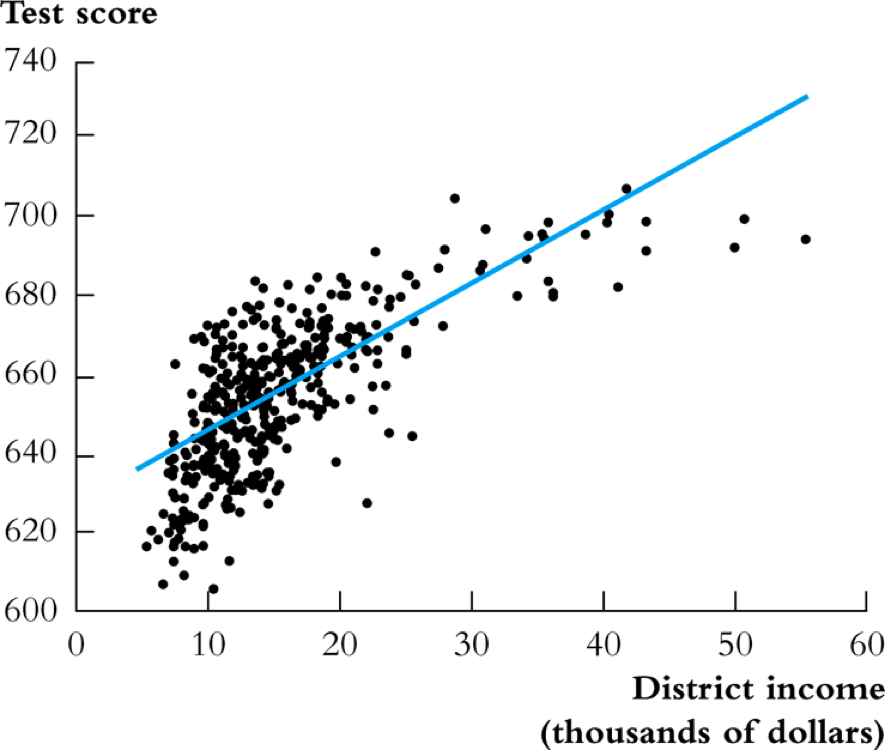
\includegraphics[width=0.85\textwidth]{img/fig-8-2.png}
\caption{\label{fig:org52d16af}
Scatterplot of test score vs district income and a linear regression line}
\end{figure}
\end{column}
\end{columns}
\end{frame}

\begin{frame}[label={sec:org9185a99}]{Why does a simple linear regression model not fit the data well?}
\begin{itemize}
\item Data points are below the OLS line when income is very low (under
\$10,000) or very high (over \$40,000), and are above the line when
income is between \$15,000 and \$30,000.

\vspace{0.1cm}
\item The scatterplot may imply a curvature in the relationship between
test scores and income. 

\vspace{0.1cm}
That is, a unit increase in income may have larger effect on test
scores when income is very low than when income is very high.

\vspace{0.1cm}
\item The linear regression line cannot capture the curvature because the
effect of district income on test scores is constant over all the
range of income since 
\[\Delta TestScore / \Delta Income = \beta_1\]
where \(\beta_1\) is constant.
\end{itemize}
\end{frame}

\begin{frame}[label={sec:orgb75e312}]{Estimate a quadratic regression model}
\begin{equation}
\label{eq:quadratic-testscore}
TestScore = \beta_0 + \beta_1 Income + \beta_2 Income^2 + u
\end{equation}

\begin{itemize}
\item This model is nonlinear, specifically quadratic, with respect to
\(Income\) since we include the squared income.

\item The population regression function is
\[E(TestScore | Income) = \beta_0 + \beta_1 Income + \beta_2 Income^2\]

\item It is linear with respect to \(\beta\). So we can still use the
OLS estimation and carry out hypothesis testing as we do with a
linear regression model.
\end{itemize}
\end{frame}

\begin{frame}[label={sec:orgf67a0aa}]{Estimate a quadratic regression model (cont'd)}
\begin{figure}[htbp]
\centering
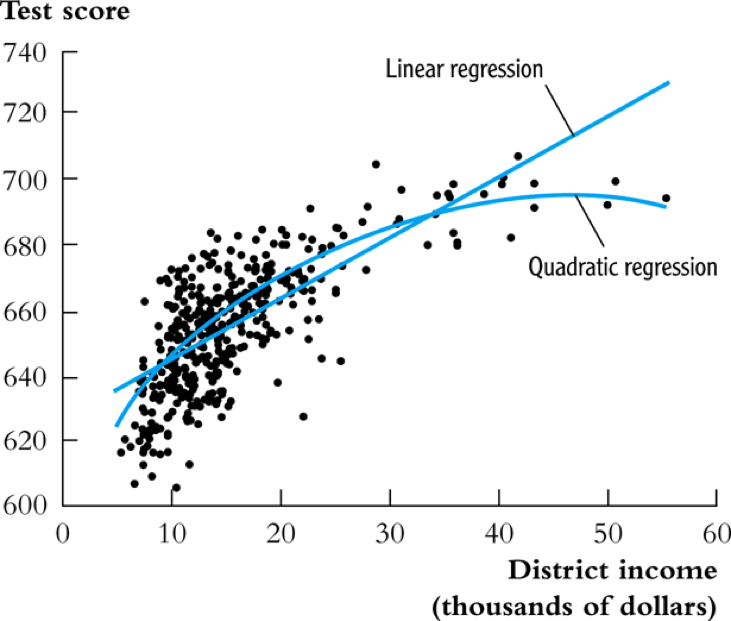
\includegraphics[width=0.6\textwidth,height=0.5\textwidth]{img/fig-8-3.png}
\caption{\label{fig:org5505e59}
Scatterplot of test score vs district income and a quadratic regression line}
\end{figure}
\end{frame}

\begin{frame}[shrink,label={sec:orgc044919}]{A general formula for a nonlinear population regression function}
A general nonlinear regression model is

\begin{equation}
\label{eq:nl-general}
Y_i = f(X_{i1}, X_{i2}, \ldots, X_{ik}; \beta_1, \beta_2, \ldots, \beta_m) + u_i
\end{equation}

\begin{itemize}
\item The \alert{population nonlinear regression function}: 
\[ E(Y_i | X_{i1}, \ldots, X_{ik}) = f(X_{i1}, X_{2i}, \ldots, X_{ik}; \beta_1, \beta_2, \ldots, \beta_m) \]
\item The number of regressors and the number of parameters are not
necessarily equal in the nonlinear regression model.
\item In vector notation 
\begin{equation}
\label{eq:nl-general-mat}
Y_i = f(\mathbf{X}_i; \boldsymbol{\beta}) + u_i
\end{equation}
\item We focus on the nonlinear regression models
such that \(f(\cdot)\) is \alert{nonlinear with \(\mathbf{X}_i\)} but \alert{linear with
\(\boldsymbol{\beta}\)}.
\end{itemize}
\end{frame}

\begin{frame}[label={sec:orgfa5aa8a}]{The effect on \(Y\) of a change in a regressor}
\begin{block}{For any general nonlinear regression function}
The effect on \(Y\) of a change in one regressor, say \(X_1\), holding
other things constant, can be computed as
\begin{equation}
\label{eq:nl-gen-effect}
\Delta Y = f(X_1 + \Delta X_1, X_2, \ldots, X_k; \boldsymbol{\beta}) - f(X_1, X_2, \ldots, X_k; \boldsymbol{\beta})
\end{equation}
\end{block}

\begin{block}{For continuous and differentiable nonlinear functions}
When \(X_1\) and \(Y\) are continuous variables and \(f(\cdot)\) is
differentiable, the marginal effect of \(X_1\) is the partial derivative
of \(f\) with respect to \(X_1\), that is, holding other things constant
\[ \mathrm{d}Y = \frac{\partial f(X_1, \ldots, X_k;
\boldsymbol{\beta})}{\partial X_i} \mathrm{d} X_i \]
because \(\mathrm{d}X_j = 0\) for \(j \neq i\)
\end{block}
\end{frame}

\begin{frame}[label={sec:org03c68bd}]{Application to test scores and income}
\begin{block}{Estimation}
\begin{equation}
\label{eq:tsr-income2}
\widehat{TestScore} = \underset{\displaystyle (2.9)}{607.3} +
\underset{\displaystyle (0.27)}{3.85}Income - \underset{\displaystyle (0.0048)}{0.0423}Income^2,\, \bar{R}^2 = 0.554
\end{equation}
\end{block}

\begin{block}{Hypothesis test}
Test \(H_0:\, \beta_2 = 0 \text{ vs. } H_1:\,\beta_2 \neq 0\). 
\[ t = \frac{-0.0423}{0.0048} = -8.81 > -1.96 \]
We reject the null at the 1\%, 5\% and 10\% significance levels, and
therefore, confirm the quadratic relationship between test scores
and income. 
\end{block}
\end{frame}

\begin{frame}[label={sec:orgc5615ed}]{The effect of change in income on test scores}
\begin{block}{A change in income from \$10 thousand to \$20 thousand}
\begin{equation*}
\begin{split}
\Delta \hat{Y} &= \hat{\beta}_0 + \hat{\beta}_1 \times 11 + \hat{\beta}_2 \times 11^2 - (\hat{\beta}_0 + \hat{\beta}_1 \times 10 + \hat{\beta}_2 \times 10^2) \\
&= \hat{\beta}_1 (11 - 10) + \hat{\beta}_2(11^2 - 10^2) \\
& = 3.85 - 0.0423 \times 21 = 2.96
\end{split}
\end{equation*}
\end{block}

\begin{block}{A change in income from \$40 thousand to \$41 thousand}
\begin{equation*}
\begin{split}
\Delta \hat{Y} &= \hat{\beta}_0 + \hat{\beta}_1 \times 41 + \hat{\beta}_2 \times 41^2 - (\hat{\beta}_0 + \hat{\beta}_1 \times 40 + \hat{\beta}_2 \times 40^2) \\
&= \hat{\beta}_1 (41 - 40) + \hat{\beta}_2(41^2 - 40^2) \\
& = 3.85 - 0.0423 \times 81 = 0.42
\end{split}
\end{equation*}
\end{block}
\end{frame}

\begin{frame}[label={sec:org1995b6f}]{A general approach to modeling nonlinearities using multiple regression}
\begin{enumerate}
\item Identify a possible nonlinear relationship.
\begin{itemize}
\item Economic theory
\item Scatterplots
\item Your judgment and experts' opinions
\end{itemize}

\item Specify a nonlinear function and estimate its parameters by OLS.
\begin{itemize}
\item The OLS estimation and inference techniques can be used as usual
when the regression function is linear with respect to \(\beta\).
\end{itemize}

\item Determine whether the nonlinear model can improve a linear model
\begin{itemize}
\item Use t- and/or F-statistics to test the null hypothesis that the
population regression function is linear against the alternative
that it is nonlinear.
\end{itemize}

\item Plot the estimated nonlinear regression function.

\item Compute the effect on \emph{Y} of a change in \emph{X} and interpret the results.
\end{enumerate}
\end{frame}


\section{Nonlinear functions of a single independent variable}
\label{sec:org986bc68}

\begin{frame}[label={sec:org8a983ba}]{Polynomials}
\begin{block}{A polynomial regression model of degree r}
\begin{equation}
\label{eq:poly-r}
Y_i = \beta_0 + \beta_1 X_i + \beta_2 X_i^2 + \cdots + \beta_r X_i^r + u_i
\end{equation}
\begin{itemize}
\item \(r = 2\): a \alert{quadratic} regression model
\item \(r = 3\): a \alert{cubic} regression model
\item Use the OLS method to estimate \(\beta_1, \beta_2, \ldots, \beta_r\).
\end{itemize}
\end{block}

\begin{block}{Testing the null hypothesis that the population regression function is linear}
\[ H_0:\, \beta_2 = 0, \beta_3 = 0, ..., \beta_r = 0 \text{ vs. }
H_1:\, \text{ at least one } \beta_j \neq 0, j = 2, \ldots, r \]

Use F statistic to test this joint hypothesis. The number of
restriction is \(q = r-1\).
\end{block}
\end{frame}

\begin{frame}[label={sec:org996b24f}]{What is \(\Delta Y / \Delta X\) in a polynomial regression model?}
\begin{itemize}
\item Consider a cubic model and continuous \(X\) and \(Y\)
\[Y = \beta_0 + \beta_1 X + \beta_2 X^2 + \beta_3 X^3 + u\]

\item Then, we can calculate
\[\frac{\dx Y}{\dx X} = \beta_1 + 2\beta_2 X + 3\beta_3 X^2 \]

\item The effect of a unit change in \(X\) on \(Y\) depends on the value of
\(X\) at evaluation.
\end{itemize}
\end{frame}

\begin{frame}[label={sec:orge443875}]{Which degree of polynomial should I use?}
\begin{itemize}
\item Balance a trade-off between flexibility and statistical precision.
\begin{itemize}
\item Flexibility. Relate Y to X in more complicated way than simple
linear regression.
\item Statistical precision. \(X, X^2, X^3, \ldots\) are correlated so
that there is the problem of imperfect multicollinearity.
\end{itemize}
\item Follow a sequential hypothesis testing procedure
\begin{enumerate}
\item Pick a maximum value of \(r\) and estimate the polynomial
regression for that \(r\).
\item Follow a "deletion" rule based on t-statistic or F-statistic.
\end{enumerate}
\end{itemize}
\end{frame}

\begin{frame}[shrink,label={sec:org709518e}]{Application to district income and test scores}
We estimate a cubic regression model relating test scores to district
income as follows
\begin{equation*}
\widehat{TestScore} = \underset{\displaystyle (5.1)}{600.1} 
                    + \underset{\displaystyle (0.71)}{5.02} Income
                    - \underset{\displaystyle (0.029)}{0.096} Income^2 
                    + \underset{\displaystyle (0.00035)}{0.00069} Income^3, \hat{R}^2 = 0.555 
\end{equation*}

\begin{block}{Test whether it is a cubic model}
The t-statistic for \(H_0: \beta_3 = 0\) is 1.97 \(\Rightarrow\) Fail to reject
\end{block}

\begin{block}{Test whether it is a nonlinear model}
The F-statistic for \(H_0: \beta_2 = \beta_3 = 0\) is 37.7, p-value
\(<0.01\)
\end{block}

\begin{block}{Interpretation of coefficients}
Use the general formula of interpreting the effect of \(\Delta X\) on
\(Y\).
\end{block}
\end{frame}

\begin{frame}[label={sec:orgebeb532}]{A natural logarithmic function \(y = \ln(x)\)}
\begin{itemize}
\item Properties of \(\ln(x)\)
\begin{gather*}
\ln(1/x) = -\ln(x),\, \ln(ax) = \ln(a) + \ln(x) \\
\ln(x/a) = \ln(x) - \ln(a),\, \text{ and } \ln(x^a) = a\ln(x)
\end{gather*}

\item The derivative of \(\ln(x)\) is
\[ \frac{\dx \ln(x)}{\dx x} = \lim_{\Delta x \rightarrow 0}
  \frac{\ln(x + \Delta x) - \ln(x)}{\Delta x} = \frac{1}{x}\,\text{.} \]
It follows that \(\dx \ln(x) = \dx x / x\), representing the percentage
change in \(x\).
\end{itemize}
\end{frame}

\begin{frame}[label={sec:orgc830afb}]{The percentage-change form using \(\ln(x)\)}
\begin{itemize}
\item The change in \(\ln(X)\) represents the percentage change in \(X\)

\[ \ln(x + \Delta x) - \ln(x) \approx \frac{\Delta x}{x} \text{ when
  } \Delta x \text{ is small.} \]

\item The Taylor expansion of \(\ln(x +
  \Delta x)\) at \(x\), which is
\begin{align*}
\ln(x + \Delta x) &= \ln(x) + \frac{\dx \ln(x)}{\dx x} (x + \Delta x - x) + \frac{1}{2!}\frac{\dx^2 \ln(x)}{\dx x^2}(x + \Delta x - x)^2 + \cdots \\
                  &= \ln(x) + \frac{\Delta x}{x} -\frac{\Delta x^2}{2x^2} + \cdots
\end{align*}
When \(\Delta x\) is very small, we can omit the terms with \(\Delta
  x^2, \Delta x^3\), etc. Thus, we have \(\ln(x + \Delta x) - \ln(x)
  \approx \frac{\Delta x}{x}\) when \(\Delta x\) is small.
\end{itemize}
\end{frame}

\begin{frame}[label={sec:org78cbb50}]{The three logarithmic regression models}
There are three types of logarithmic regression models:

\begin{itemize}
\item Linear-log model

\item Log-linear model

\item Log-log model
\end{itemize}

Differences in logarithmic transformation of \(X\) and/or \(Y\) lead to
differences in interpretation of the coefficient.
\end{frame}

\begin{frame}[label={sec:orgecab655}]{Case I: linear-log model}
\begin{itemize}
\item \alert{Model form}. \(X\) is in logarithms, \(Y\) is not.
\begin{equation}
\label{eq:linear-log}
Y_i = \beta_0 + \beta_1 \ln(X_i) + u_i, i = 1, \ldots, n
\end{equation}

\item \alert{Interpretation}. a 1\% change in \(X\) is associated with a
change in \(Y\) of 0.01\(\beta_{\text{1}}\)
\[ \Delta Y = \beta_1 \ln(X + \Delta X) - \beta_1 \ln(X) \approx
  \beta_1 \frac{\Delta X}{X} \]

\item \alert{Example}. The estimated model is 
\[\widehat{TestScore} = 557.8 + 36.42\ln(Income)\] 
\begin{itemize}
\item 1\% increase in average district income results in an increase in
test scores by \(0.01 \times 36.42 = 0.36\) point.
\end{itemize}
\end{itemize}
\end{frame}

\begin{frame}[label={sec:orge8a603f}]{Case II: log-linear model}
\begin{itemize}
\item \alert{Model form}. \(Y\) is in logarithms, \(X\) is not.
\begin{equation}
\label{eq:log-linear}
\ln(Y_i) = \beta_0 + \beta_1 X_i + u_i
\end{equation}

\item \alert{Interpretation}. A one-unit change in \(X\)
is associated with a \(100 \times \beta_1\%\) change in \(Y\) because
\begin{equation*}
\frac{\Delta Y}{Y} \approx \ln(Y + \Delta Y) - \ln(Y) = \beta_1 \Delta X
\end{equation*}

\item \alert{Example}. 
\[ \widehat{\ln(Earnings)} = 2.805 + 0.0087Age \]
\begin{itemize}
\item Earnings are predicted to increase by 0.87\% for each additional
year of age.
\end{itemize}
\end{itemize}
\end{frame}

\begin{frame}[shrink,label={sec:orgca2ccde}]{Case III: log-log model}
\begin{itemize}
\item \alert{Model form}. Both \(X\) and \(Y\) are in logarithms.
\begin{equation}
\label{eq:log-log}
\ln(Y_i) = \beta_0 + \beta_1 \ln(X_i) + u_i
\end{equation}

\item \alert{Interpretation: elasticity}. 1\% change in \(X\) is associated with a
\(\beta_{\text{1}}\)\% change in \(Y\) because 
\begin{equation*}
\frac{\Delta Y}{Y} \approx \ln(Y +
\Delta Y) - \ln(Y) = \beta_1 (\ln(X + \Delta X) - \ln(X)) \approx
\beta_1 \frac{\Delta X}{X}
\end{equation*}

\begin{itemize}
\item \(\beta_{\text{1}}\) is the \alert{elasticity} of \(Y\) with respect to \(X\), that is 
\[ \beta_1 = \frac{100 \times
    (\Delta Y / Y)}{100\times (\Delta X / X)} =\frac{\text{percentage
    change in } Y}{\text{percentage change in } X} \]
\item With the derivative, \(\beta_1 = \dx \ln(Y) / \dx \ln(X) = (\dx Y/Y)
    / (\dx X/X)\).
\end{itemize}

\item \alert{Example}. The log-log model of the test score application is
estimated as
\[ \widehat{\ln(TestScore)} = 6.336 + 0.0544 \ln(Income) \]
This implies that a 1\% increase in income corresponds to a
0.0544\% increase in test scores.
\end{itemize}
\end{frame}

\begin{frame}[label={sec:orgd3f68f7}]{The log-linear and log-log regression functions}
\begin{figure}[htbp]
\centering
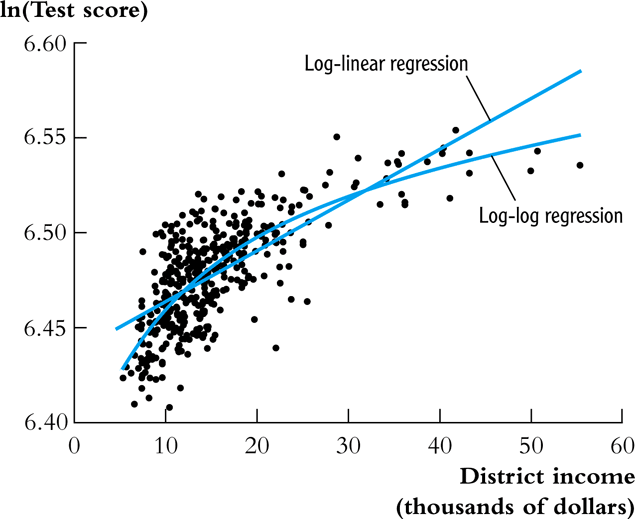
\includegraphics[width=0.65\textwidth]{img/fig-8-6.png}
\caption{\label{fig:org31fabba}
The log-linear and log-log regression functions}
\end{figure}
\end{frame}

\begin{frame}[label={sec:org2ebdcdb}]{Summary}
\begin{center}
\begin{tabular}{p{4cm}p{6cm}}
Regression specification & Interpretation of \(\beta_1\)\\
\hline
\(Y = \beta_0 + \beta_1 \ln(X) + u\) & A 1\% change in X is associated with a change in Y of \(0.01\beta_{1}\)\\
\hline
\(\ln(Y) = \beta_0 + \beta_1 X + u\) & A change in X by one unit is associated with a \(100\beta_1\%\) change in Y\\
\hline
\(\ln(Y) = \beta_0 + \beta_1 \ln(X) + u\) & A 1\% change in X is associated with a \(\beta_{1}\%\) change in Y, so \(\beta_1\) is the elasticity of Y with respect to X\\
\end{tabular}
\end{center}
\end{frame}


\section{Interactions between independent variables}
\label{sec:orgfb1645c}

\begin{frame}[label={sec:org4045bc6}]{Interactions between independent variables}
\begin{itemize}
\item Interaction between two binary variables

\vspace{0.1cm}

\item Interaction between a continuous and a binary variable

\vspace{0.1cm}

\item Interaction between two continuous variables
\end{itemize}
\end{frame}

\begin{frame}[label={sec:orgf1773e1}]{The regression model with interaction between two binary variables}
\begin{block}{Two binary variables}
\begin{itemize}
\item \(D_{1i} = 1\) if the i\(^{\text{th}}\) person has a college degree, and 0 otherwise.
\item \(D_{2i} = 1\) if the i\(^{\text{th}}\) person is female, and 0 otherwise.
\end{itemize}
\end{block}

\begin{block}{A regression with an interaction term of two binary variables}
Consider a regresion model concerning the effects of education and
gender on earnings. The population regression function is
\begin{equation}
\label{eq:interact-dd}
Y_i = \beta_0 + \beta_1 D_{1i} + \beta_2 D_{2i} + \beta_3 (D_{1i} \times D_{2i}) + u_i
\end{equation}
\begin{itemize}
\item The dependent variable: \(Y_i\), where \(Y_i = Earnings_i\)
\item \(D_{1i} \times D_{2i}\) is the \alert{interaction term}.
\end{itemize}
\end{block}
\end{frame}

\begin{frame}[label={sec:org01fa192}]{The method of interpreting coefficients in regressions with interacted binary variables}
We can follow a general rule for interpreting coefficients in Equation
(\ref{eq:interact-dd}):

\begin{itemize}
\item First compute the expected values of \(Y\) for each possible case
described by the set of binary variables.

\vspace{0.1cm}

\item Next compare these expected values. Each coefficient can then be
expressed either as an expected value or as the difference between
two or more expected values.
\end{itemize}
\end{frame}

\begin{frame}[label={sec:org4a06a60}]{Compute the expected values of \(Y\) for each possible combinations of \(D_1\) and \(D_2\)}
\begin{description}
\item[{Case 1}] \(E(Y_i | D_{1i} = 0, D_{2i} = 0) = \beta_0\): the average
income of male non-college graduates.

\item[{Case 2}] \(E(Y_i | D_{1i} = 1, D_{2i} = 0) = \beta_0 + \beta_1\):
the average income male college graduates.

\item[{Case 3}] \(E(Y_i | D_{1i} = 0, D_{2i} = 1) = \beta_0 + \beta_2\): the
average income of female non-college graduates.

\item[{Case 4}] \(E(Y_i | D_{1i} = 1, D_{2i} = 1) = \beta_0 + \beta_1 +
            \beta_2 + \beta_3\): the average income of female college
graduates.
\end{description}
\end{frame}

\begin{frame}[label={sec:org2c172f5}]{Compute the difference between a pair of cases}
\begin{description}
\item[{Case 1 vs. Case 2}] \(E(Y_i | D_{1i} = 1, D_{2i} = 0) - E(Y_i |
     D_{1i} = 0, D_{2i} = 0) = \beta_1\): the average income
difference between college graduates and non-college graduates among
male workers.

\item[{Case 1 vs. Case 3}] \(E(Y_i | D_{1i} = 0, D_{2i} = 1) - E(Y_i |
     D_{1i} = 0, D_{2i} = 0) = \beta_2\):  the average income
difference between female and male workers who are not college
graduates.

\item[{Case 1 vs. Case 4}] \(E(Y_i | D_{1i} = 1, D_{2i} = 1) - E(Y_i |
     D_{1i} = 0, D_{2i} = 0) = \beta_1 + \beta_2 + \beta_3\): the
average income difference between female college graduates and
male non-college graduates.
\end{description}
\end{frame}

\begin{frame}[label={sec:org89aca50}]{Compute the difference between a pair of cases (cont'd)}
\begin{description}
\item[{Case 2 vs. Case 3}] \(E(Y_i | D_{1i} = 0, D_{2i} = 1) - E(Y_i |
     D_{1i} = 1, D_{2i} = 0) = \beta_2 - \beta_1\). Thus, the average
income difference between female non-college graduates and male
college graduates is \(\beta_2 - \beta_1\).

\item[{Case 2 vs. Case 4}] \(E(Y_i | D_{1i} = 1, D_{2i} = 1) - E(Y_i |
     D_{1i} = 1, D_{2i} = 0) = \beta_2 + \beta_3\). Thus, the average
income difference between female college graduates and male
college graduates is \(\beta_2 + \beta_3\).

\item[{Case 3 vs. Case 4}] \(E(Y_i | D_{1i} = 1, D_{2i} = 1) - E(Y_i |
     D_{1i} = 0, D_{2i} = 1) = \beta_1 + \beta_3\). Thus, the average
income difference between female college graduates and female
non-college graduates is \(\beta_1 + \beta_3\).
\end{description}
\end{frame}

\begin{frame}[label={sec:org06b3c9a}]{Hypothesis testing}
We can use t-statistic or F-statistic to test whether the differences
between different cases are statistically significant.

\begin{block}{The null hypothesis: \(H_0: \beta_2 = 0 \text{ vs. } H_1: \beta_2 \neq 0\).}
\begin{itemize}
\item What is this test for?
\item What test statistic can we use?
\end{itemize}
\end{block}

\begin{block}{The hypothesis is \(H_0: \beta_1 + \beta_3 = 0 \text{ vs. } H_1: \beta_1 + \beta_3 \neq 0\).}
\begin{itemize}
\item What is this test for?
\item What test statistic can we use?
\end{itemize}
\end{block}
\end{frame}

\begin{frame}[label={sec:org3469247}]{Interactions between a continuous and a binary variable}
Consider the population regression of earnings (\(Y_i\)) against
\begin{itemize}
\item one continuous variable, individual's years of work experience
(\(X_i\)), and
\item one binary variable, whether the worker has a college degree
(\(D_i\), where \(D_i=1\) if the i\(^{\text{th}}\) person is a college graduate).
\end{itemize}

\vspace{0.3cm}
As shown in the next figure, the population regression line relating \(Y\) and
\(X\) can depend on \(D\) in three different ways.
\end{frame}

\begin{frame}[label={sec:orgc9ca817}]{Interactions between a continuous and a binary variable: graphic representation}
\begin{figure}[htbp]
\centering
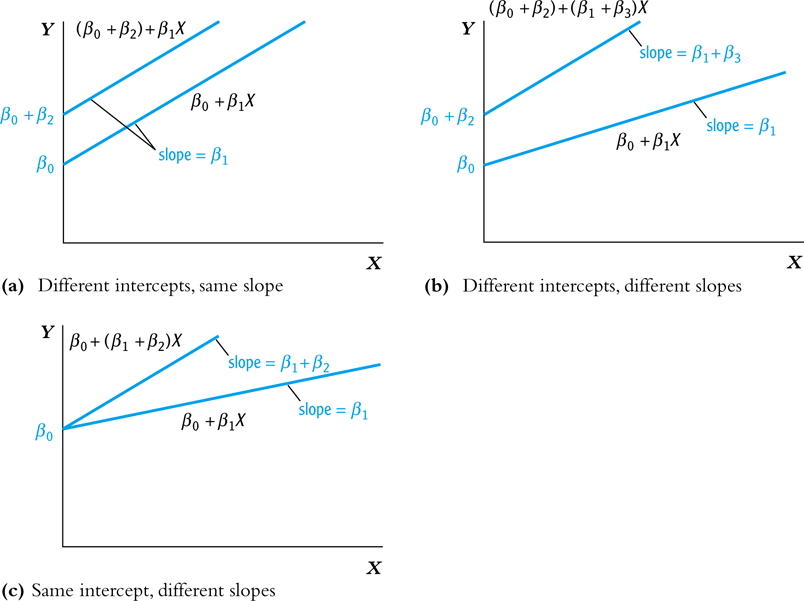
\includegraphics[width=0.75\textwidth]{img/fig-8-8.png}
\caption{\label{fig:orgd267b58}
Regression Functions Using Binary and Continuous Variables}
\end{figure}
\end{frame}

\begin{frame}[label={sec:orgb6c5195}]{Different intercept, same slope: (a) in Figure \ref{fig:orgd267b58}}
\begin{equation}
\label{eq:interact-dx-a}
Y_i = \beta_0 + \beta_1 X_i + \beta_2 D_i + u_i
\end{equation}

\begin{itemize}
\item From Equation (\ref{eq:interact-dx-a}), we have the population
regression functions as
\begin{itemize}
\item \(E(Y_i | D_i = 1) = (\beta_0 + \beta_2) + \beta_1 X_i\)
\item \(E(Y_i | D_i = 0) = \beta_0 + \beta_1 X_i\).
\end{itemize}
Thus, \(E(Y_i | D_i = 1) - E(Y_i | D_i = 0) = \beta_2\).

\item The average initial salary of college graduates is higher than
non-college graduates by \(\beta_2\), and this gap persists at the same
magnitude regardless of how many years a worker has been working.
\end{itemize}
\end{frame}

\begin{frame}[label={sec:org412e1bc}]{Different intercepts and different slopes: (b) in Figure \ref{fig:orgd267b58}}
Equation (\ref{eq:interact-dx-a}):
\begin{equation}
\label{eq:interact-dx-b}
Y_i = \beta_0 + \beta_1 X_i + \beta_2 D_i + \beta_3 (X_i \times D_i) + u_i
\end{equation}

\begin{itemize}
\item The population regression functions for the two cases are
\begin{itemize}
\item \(E(Y_i|D_i=1) = (\beta_0+\beta_2) + (\beta_1 + \beta_3) X_i\)
\item \(E(Y_i|D_i=0) = \beta_0 + \beta_1 X_i\).
\end{itemize}
Thus, \(\beta_2\) is the difference in intercepts and \(\beta_3\) is the
difference in slopes.

\item The average initial salary of college graduates is higher than
non-college graduates by \(\beta_2\), and this gap will widen (or
narrow) depending on the effect of the years of work experience on
earnings.
\end{itemize}
\end{frame}

\begin{frame}[label={sec:org07c9b35}]{Different intercepts and same intercept: (c) in Figure \ref{fig:orgd267b58}}
\begin{equation}
\label{eq:interact-dx-c}
Y_i = \beta_0 + \beta_1 X_i + \beta_2 (X_i \times D_i) + u_i
\end{equation}

\begin{itemize}
\item The population regression functions for the two cases are
\begin{itemize}
\item \(E(Y_i|D_i=1) = \beta_0 + (\beta_1 + \beta_2) X_i\)
\item \(E(Y_i|D_i=0) = \beta_0 + \beta_1 X_i\).
\end{itemize}
Thus, there is only a difference in the slope but not in the
intercept.

\item Although college graduates have the same starting salary as those
withou colledge degree, the raise in salary and promotion of the
former will be faster than the latter.
\end{itemize}
\end{frame}

\begin{frame}[label={sec:org7c9c304}]{Interactions between two continuous variables}
Now we consider the regression of earnings against two continuous
variables, one for the years of work experience (\(X_1\)) and another
for the years of schooling (\(X_2\)).

\vspace{0.2cm}
The interaction model is
\begin{equation}
\label{eq:interact-xx}
Y_i = \beta_0 + \beta_1 X_{1i} + \beta_2 X_{2i} + \beta_3 (X_{1i} \times X_{2i}) + u_i
\end{equation}
\begin{itemize}
\item The effect of a change in \(X_1\), holding \(X_2\) constant, is

\[ \frac{\Delta Y}{\Delta X_1} = \beta_1 + \beta_3 X_2 \]
\item Similarly, the effect of a change in \(X_2\), holding \(X_1\) constant, is
\[ \frac{\Delta Y}{\Delta X_2} = \beta_1 + \beta_3 X_1 \]
\end{itemize}
\end{frame}


\section{Warm-up exercises}
\label{sec:org0381032}

\begin{frame}[label={sec:org7f8451c}]{Question 1}
The interpretation of the slope coefficient in the model \(\ln(Y_i) =
\beta_0 + \beta_1 \ln(X_i)+ u_i\) is as follows:
\begin{description}
\item[{A)}] a 1\% change in X is associated with a \(\beta_{\text{1}}\)\% change in Y.
\item[{B)}] a change in X by one unit is associated with a \(\beta_{\text{1}}\) change in Y.
\item[{C)}] a change in X by one unit is associated with a 100 \(\beta_{\text{1}}\) \% change in Y.
\item[{D)}] a 1\% change in X is associated with a change in Y of 0.01\(\beta_{\text{1}}\).
\end{description}
\pause
Answer: A
\end{frame}

\begin{frame}[label={sec:orge291d30}]{Question 2}
In the regression model \(Y_i = \beta_0 + \beta_1 X_i + \beta_2 D_i +
\beta_3 (X_i \times D_i) + u_i\), where X is a continuous variable and
D is a binary variable, to test that the two regressions are
identical, you must use the
\begin{description}
\item[{A)}] t-statistic separately for \(\beta_2 = 0, \beta_3 = 0\).
\item[{B)}] F-statistic for the joint hypothesis that \(\beta_0 = 0,
        \beta_1 = 0\)
\item[{C)}] t-statistic separately for \(\beta_3 = 0\)
\item[{D)}] F-statistic for the joint hypothesis that \(\beta_2 = 0,
        \beta_3 = 0\).
\end{description}
\pause
Answer:  D

\pause
\end{frame}
\begin{frame}[label={sec:orgf178908}]{Question 3}
(Requires Calculus)  In the equation \(\widehat{TestScore} = 607.3 +
3.85 Income - 0.0423 Income^2\), the following income level results in
the maximum test score
\begin{description}
\item[{A)}] 607.3.
\item[{B)}] 91.02.
\item[{C)}] 45.50.
\item[{D)}] cannot be determined without a plot of the data.
\end{description}
\pause
Answer:  C
\end{frame}


\section{Regression Functions That Are Nonlinear in the Parameters}
\label{sec:org56564b0}
\begin{frame}[label={sec:org9cc3248}]{Nonlinear regression models and nonlinear least squares estimator}
All the regression models that we have discussed in this lecture are
nonlinear in the regressors but linear in parameters so that we can
still treat them as linear regression models and estimate using the
OLS.

\vspace{0.1cm}

However, there exist regression models that are nonlinear in
parameters. For these models, we can either transform them to the
"linear" type of models or estimate using the \alert{nonlinear least
squares} (NLS) estimators.
\end{frame}

\begin{frame}[label={sec:org7ba055d}]{Transform a nonlinear model to a linear one}
Suppose we have a nonlinear regression model as follows
\begin{equation}
\label{eq:nls-xaxb}
Y_i =  \alpha X_{1i}^{\beta_1}X_{2i}^{\beta_2}\cdots X_{ki}^{\beta_k}e^{u_i}
\end{equation}

\vspace{0.1cm}

Taking the natural logarithmic function on both sides
of the equation
\begin{equation}
\label{eq:nls-linear-xaxb}
\ln(Y_i) = \ln(\alpha) + \beta_1 \ln(X_{1i}) + \beta_2 \ln(X_{2i}) + \cdots + \beta_k \ln(X_{ki}) + u_i
\end{equation}
\begin{itemize}
\item Equation (\ref{eq:nls-xaxb}) becomes a log-log regression model,
which is linear in all parameters and can be estimated using the
OLS. Let \(\beta_0 = \ln(\alpha)\) and \(\alpha = e^{\beta_0}\).
\item \(\beta_i\) for \(i=1, 2, \ldots, k\) are the elasticities of \(Y\) with
respect to \(X_i\).
\end{itemize}
\end{frame}

\begin{frame}[shrink,label={sec:orgd05e98e}]{A nonlinear model: logistic function}
\begin{itemize}
\item A dependent variable can only take values between 0 and 1.
\end{itemize}

\vspace{0.3cm}

\begin{itemize}
\item The logistic regression model with k regressors is
\begin{equation}
\label{eq:logistic}
Y_i = \frac{1}{1 + \exp(\beta_0 + \beta_1 X_{1i} + \cdots \beta_k X_{ki})} + u_i
\end{equation}

\begin{itemize}
\item For small values of \(X\), the value of the function is nearly 0 and
the shape is flat.
\item For large values of \(X\), the function approaches 1 and the slope is
flat again.
\end{itemize}
\end{itemize}
\end{frame}

\begin{frame}[label={sec:org4d9d414}]{A nonlinear model: negative exponential growth function}
\begin{itemize}
\item The effect of \(X\) on \(Y\) must be positive and the effect is
bounded by a upper bound.

\item Use the negative-exponential growth function to set up a regression model as follows
\begin{equation}
\label{eq:neg-exp}
Y_i = \beta_0 [1-\exp(-\beta_1(X_i - \beta_2))] + u_i
\end{equation}

\begin{itemize}
\item The slope is positive for all values of \(X\).
\item The slope is greatest at low values of \(X\) and decreases as \(X\)
increases.
\item There is an upper bound, that is, a limit of \(Y\) as \(X\) goes to
infinity, \(\beta_0\).
\end{itemize}
\end{itemize}
\end{frame}

\begin{frame}[label={sec:org54e1d37}]{Logistic and negative exponential growth curves}
\begin{figure}[htbp]
\centering
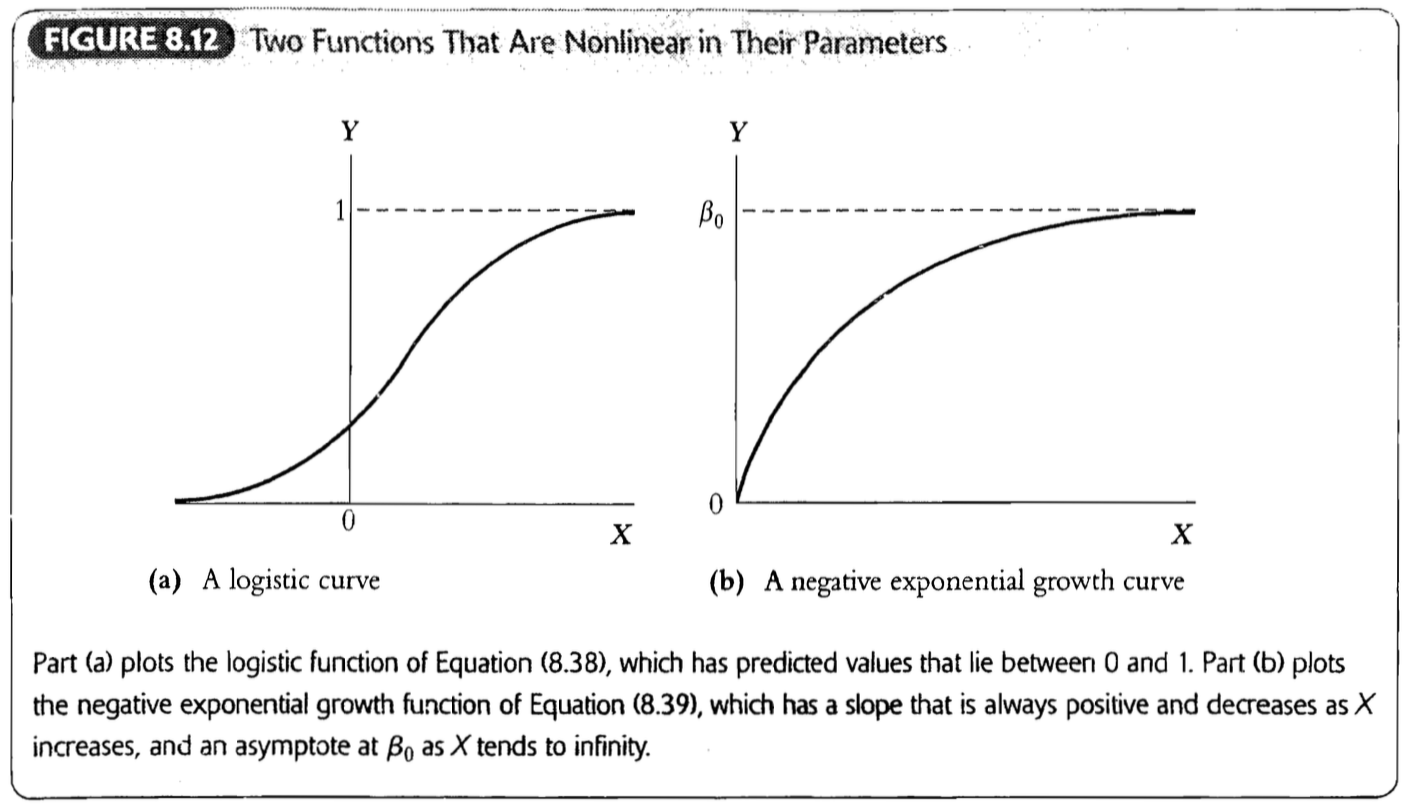
\includegraphics[width=.9\linewidth]{img/fig-8-12.png}
\caption{\label{fig:org0ec3b21}
The logistic and negative exponential growth functions}
\end{figure}
\end{frame}

\begin{frame}[label={sec:org4bbc184}]{The nonlinear least squares estimators}
For a nonlinear regression function
\[ Y_i = f(X_1, \ldots, X_k; \beta_1, \ldots, \beta_m) + u_i \]
which is nonlinear in both \(X\) and \(\beta\), we can obtain the
estimated parameters by \alert{nonlinear least squares} (NLS) estimation. 

\vspace{0.1cm}

The essential idea of NLS is the same as OLS, which is to minimize the sum
of squared prediction mistakes. That is
\begin{equation*}
\operatorname*{min}_{b_1, \ldots, b_m}\: S(b_1, \ldots, b_m) = \sum_{i=1}^n \left[ Y_i - f(X_1, \ldots, X_k; b_1, \ldots, b_m) \right]^2
\end{equation*}
The solution to this minimization problem is the nonlinear least
squares estimators.
\end{frame}
\end{document}